\documentclass[a4paper,11pt]{scrartcl}

\usepackage{vorschule}
\usepackage[
	typ=ab,
	fach=Informatik,
	lerngruppe={Diff 8},
	module={Lizenzen},
	lizenz={cc-by-nc-sa-4},
]{schule}

\usepackage[
	kuerzel=Ngb,
	reihe={Webseiten erstellen mit HTML},
	version={0.1 (2018)},
	url={https://www.github.com/jneug/schule},
]{ngbschule}

\author{J. Neugebauer}
\title{Grundstruktur einer HTML Seite}
\date{\Heute}

\setzeAufgabentemplate{ngbnormal}

\begin{document}
\ReiheTitel

\begin{quote}
HTML steht für \enquote{Hypertext Markup Language}. HTML ist eine formale Sprache zur Beschreibung der Struktur von Hypertexten (in Form verlinkter Webseiten) mit Hilfe von Auszeichnungen.
\end{quote}

\begin{aufgabe}
Ruft die Adresse \url{https://link.ngb.schule/html-bailey} im Firefox Browser auf. Unten ist der Quelltext der Seite abgebildet. Studiert den Quelltext und vergleicht ihn mit der Darstellung der Seite im Browser. Beantwortet dann folgende Fragen:
\begin{smallenumerate}
	\item  Wieso ist HTML eine \enquote{Auszeichnungssprache}?
	\item Welche Elemente erkennt ihr?
	\item Welche Grundstruktur hat eine HTML-Seite?
\end{smallenumerate}
\begin{lstlisting}[language=HTML,basicstyle=\scriptsize\ttfamily]
<!doctype html>
<html>
<head>
	<meta charset="utf-8">
	<link href='styles/style.css' rel='stylesheet' type='text/css'>
	<title>Homepage von Bailey</title>
</head>
<body>
	<h1>Hallo, ich heiße Bailey</h1>
	<p>
	<img src="img/bailey1.jpg" alt="Foto von Bailey">
	</p>
	<p>
	Hallo, ich heiße Bailey und lebe in der Nähe von 
	<a href="http://www.kaiserslautern.de">Kaiserslautern</a>. 
	Ich bin ein Australian Shepherd, meine Vorfahren haben in 
	Australien Schafe gehütet.
	</p>
	<p>
	Wenn ich erwachsen bin, will ich Agility-Sport treiben. 
	Wisst ihr überhaupt, was das ist? Wenn nicht, dann schaut 
	euch doch mal die Fotos bei 
	<a href="https://de.wikipedia.org/wiki/Agility">Wikipedia</a> 
	an. Ihr werdet staunen, was wir Hunde alles können!
	</p>
	<p>
	Ich kann aber auch schon ganz viel. Das könnt ihr auf 
	der <a href="_bailey2.html">nächsten Seite</a> sehen.
	</p>
</body>
</html>
\end{lstlisting}
\end{aufgabe}

\begin{aufgabe}
	\begin{wrapfigure}{r}{3cm}
		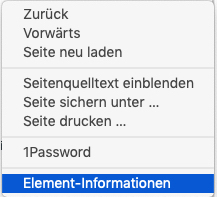
\includegraphics[width=3cm]{01-Abb_Menu.jpg}
	\end{wrapfigure}
	Durch einen Rechtsklick im Browserfenster könnt ihr ein \menu{Element untersuchen} und sogar \enquote{live} bearbeiten. Nutzt diesen \enquote{Inspektor}, um die Seite weiter zu erkunden.
\end{aufgabe}

\end{document}